\documentclass[8pt, mathserif, notheorems]{beamer}
\usetheme{Frankfurt}
\usecolortheme{spruce}

\usepackage{macrosabound, theorem-env}

\setbeamertemplate{theorems}[numbered] % number theorems
\setbeamertemplate{footline}[frame number] % number slides
\setbeamertemplate{navigation symbols}{}
\setbeamercolor{block title}{bg=blue!21,fg=black}
\setbeamertemplate{bibliography item}{\insertbiblabel}
\setbeamertemplate{itemize item}{\color{black}$\bullet$}
\setbeamertemplate{enumerate items}[default]

\usepackage{amssymb,amsmath,amsthm,enumerate,verbatim,fancyhdr,tcolorbox}
\usepackage{ulem}
\usepackage{biblatex}

% use mathptmx pkg while using default mathcal font
\DeclareMathAlphabet{\mathcal}{OMS}{cost}{m}{n}

\newcommand*{\mybox}[1]{\framebox{#1}}

\makeatother
\newlength{\colwidth}
\setlength{\colwidth}{0.5\textwidth}

\setbeamersize{text margin left=1em,text margin right=1em} 

\renewcommand{\headrulewidth}{0pt}
\graphicspath{ {./images/} }
\addbibresource{bib.bib}
\title{Theoretical Formulation of the General Reverse Ising Problem and Fast Algorithmic Solutions}
\author{Isaac Martin and Andrew Moore}
\institute{University of Texas at Austin}
\date{\today}

\begin{document}
\frame{\titlepage}

\section{Terminology}
\begin{frame}[t]\frametitle{Circuits}
  Fix the following data:
  \begin{itemize}
    \item $X$ some arbitrary index set
    \item $\Sigma = \{-1,1\}$ the set of possible spin states (switch between $\{0,1\}$ and $\{-1,1\}$ conventions via $x \mapsto 2x - 1$).
  \end{itemize}
  \bigskip

We define a \textbf{circuit} to be a tuple $(N,M,f)$ where
    \begin{itemize}    
        \item $N, M \subseteq X$ are arbitrary finite disjoint subsets of $X$. We call $N$ the collection of \textit{input} indices or vertices and $M$ the collection of \textit{output} indices/vertices.
        \item $f: \Sigma^N \to \Sigma^M$ is an arbitrary function -- the \textit{logic} of the circuit.
    \end{itemize}    
    \bigskip

    Additionally,
    \begin{itemize}
      \item $\Sigma^X$ is the collection of functions $X\to \Sigma$. It is isomorphic to $\overbrace{\Sigma\times ...\times \Sigma}^{|X| ~\text{ times}}$; tuples valued in $\Sigma$ with $|X|$ many components. We call $\Sigma^X$ the \textbf{spin space} or \textbf{state space} of $X$.
      \item $\Sigma^N$ is the \textbf{input spin space}.
      \item $\Sigma^M$ is the \textbf{output spin space}.
    \end{itemize}
\end{frame}
\begin{frame}[c]\frametitle{Ising Systems}

  An \textbf{Ising system} is a pair $(X, H)$, often referred to as simply $X$, where

  \bigskip

  \begin{itemize}
    \item $X$ is the set from the previous slide, often a subset of $\bN$ 
        \bigskip

    \item $H \in \bR[X]$ is a multilinear quadratic polynomial in elements of $X$ called the \textit{Hamiltonian} of the Ising system.
  \end{itemize}

  \bigskip

  The \textbf{state space} of $X$ is $\Sigma^X$. An Ising system $X$ in state $\sigma \in \Sigma^X$ has energy $H(\sigma)$ given by evaluating the Hamiltonian at $\sigma$.
\end{frame}
\begin{frame}\frametitle{Picture of Circuits and Systems}
  
\end{frame}
\begin{frame}[t]\frametitle{Reverse Ising Problem: Solving Circuits with Ising Systems}
We would like to design Ising systems $(X,H)$ with the following features:
\begin{enumerate}[(1)]
  \item A subset $N \subseteq X$ of spins whose state can be fixed
  \item A subset $M \subseteq X$ whose states vary freely with dynamics
  \item For a choice $\sigma_N \in \Sigma^N$, the most likely spin state in $\sigma_M \in \Sigma^M$ is $f(\sigma_N)$, where $f: \Sigma^N \to \Sigma^M$ is some function.
\end{enumerate}

Doing so for an arbitrary circuit is called \textbf{solving the reverse Ising problem}. Stated another way:
\bigskip

\textbf{Reverse Ising Problem:} Decompose $X$ as $X = N \cup M \cup A$ so that $\Sigma^X = \Sigma^N \times \Sigma^M\times \Sigma^A$. Given an abstract circuit $(N,M,f)$, design an Ising system $(X,H)$ such that for every choice of input state $\sigma \in \Sigma^N$, there is some $\eta \in \Sigma^A$ such that
\begin{align*}
  H(\sigma, f(\sigma), \eta) < H(\sigma, \omega, \eta') ~ \text{ whenever } ~ \omega \neq f(\sigma).
\end{align*}
In this situation we say that $(X,H)$ \textit{solves} the circuit $(N,M,f)$.
\end{frame}
\begin{frame}[c]\frametitle{More terminology}
  \begin{itemize}
    \item We often let $A = X \setminus (N\cup M)$ be the set of \textbf{auxiliary} spins.

      \bigskip

    \item For each input spin state $\sigma \in \Sigma^N$ we call $\{\sigma\} \times \Sigma^{M \cup A}$ the \textit{input level} of $\sigma$. This is verbally useful -- an Ising system $(X,H)$ solves a circuit $(N,M,f)$ if the correct output $f(\sigma)$ is the \textit{minimizer of its input level.}
  \end{itemize}
\end{frame}
\begin{frame}[t]\frametitle{Examples}
  \begin{minipage}{0.49\textwidth}
  \begin{center}
    \Large \underline{AND}
  \end{center}
  \end{minipage}
  \begin{minipage}{0.49\textwidth}
  \begin{center}
    \Large \underline{XOR}
  \end{center}  
  \end{minipage}
\end{frame}
\begin{frame}[c]\frametitle{Dynamics and our Goal}
  We are only interested in finding Ising systems such that the correct answer of each input minimizes the Hamiltonian on its input level. This does \textit{not} necessarily yield good dynamics, but it is a necessary condition for good dynamics to be present.

  \bigskip

 \textbf{Our Goal:} Find robust methods for algorithmically finding Ising systems which solve arbitrary circuits. Work on dynamics later.
\end{frame}

\section{Pseudo Boolean Results}
\begin{frame}[t]
  XOR is the first example of a circuit which is infeasible without auxiliaries. This is common -- an Ising Hamiltonian only has access to quadratic terms and is hence not especially expressive.

  \bigskip

  What would a \textbf{higher degree Hamiltonian} look like?
\end{frame}
\begin{frame}[t]\frametitle{All Circuits are Solvable via Higher Degree Hamiltonians}
  \begin{prop}
    Any circuit $(N,M,f)$ can be solved without auxiliaries by a multilinear polynomial $H$ of high enough degree.
  \end{prop}

  \bigskip

  \textbf{Key Fact:} Any pseudo boolean function $g:\Sigma^X \to \bR$ can be uniquely represented by a multilinear polynomial \cite{boroshammer}.

  \bigskip

  \textit{Proof:}
\end{frame}
\begin{frame}[c]\frametitle{Fourier/Hadamard Transform}
  \textbf{Note:} Given a pseudo-Boolean function $g:\Sigma^X \to \bR$, the unique multilinear polynomial representation of $g$ is actually the \textit{Hadamard Transform of $g$}, a type of generalized Fourier transform.
\end{frame}
\begin{frame}[t]\frametitle{Rosenberg Reduction}
  These higher degree Hamiltonians can actually be reduced to quadratic polynomials at the cost of adding auxiliary variables using \textbf{Rosenberg reduction.}

  \bigskip

  \textbf{Observation:} For $x,y,z \in \{0,1\}$ the following equivalences hold:
  \begin{itemize}
    \item $xy = z$ iff $xy - 2xz - 2yz + 3z = 0$
    \item $xy \neq z$ iff $xy - 2xz - 2yz + 3z > 0$.
  \end{itemize}

  \bigskip

  Rosenberg reduction works by replacing products with new auxiliary variables and penalizing ``incorrect'' values of the new variables.

  \bigskip

  \textbf{Example:} Let $f(x_1,x_2,x_3) = x_1x_2x_3$. This has minimum value at $x_1 = x_2 = x_3 = 0$.
\end{frame}
\begin{frame}[t]\frametitle{Full Rosenberg Algorithm}
  \begin{center}
    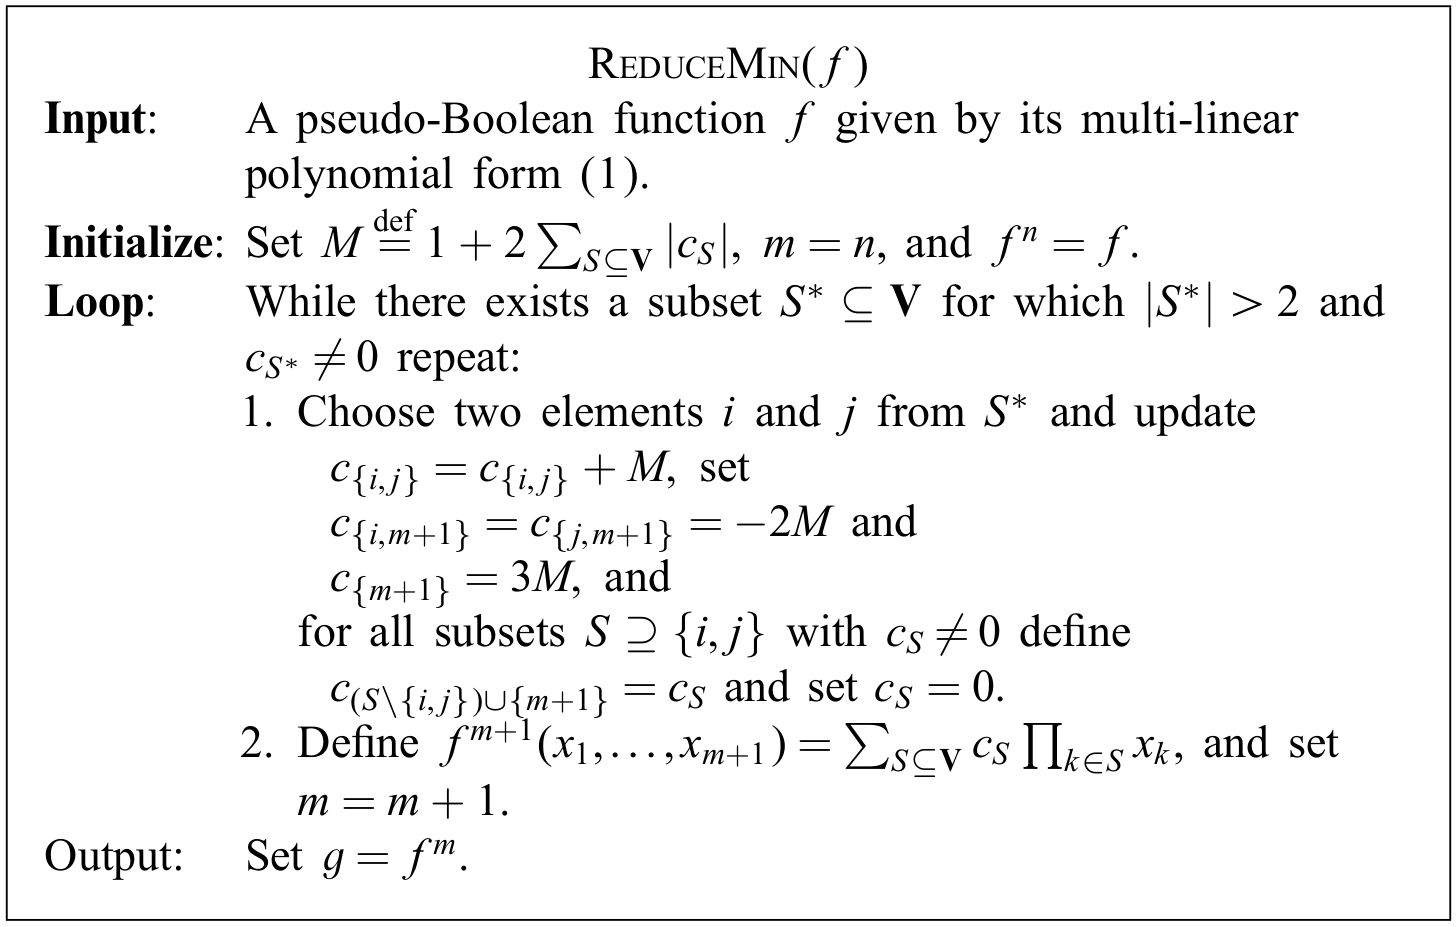
\includegraphics[width=1\textwidth]{images/rosenberg-algo.png}
  \end{center}
\end{frame}
\begin{frame}[t]\frametitle{All circuits solvable with auxiliaries}
  \begin{prop}\label{prop:all-circuits-solvable-with-auxiliaries}
    Any circuit $(N,M,f)$ can be solved by an Ising system $(X,H)$ with finitely many auxiliaries.
  \end{prop}
Notice that this lemma says nothing about the \textit{number} of auxiliary spins needed to solve a circuit; in general, it can be quite large.
\begin{proof}
  Take the hamming objective function from before:
  \begin{align*}
    g(\sigma_N, \sigma_M) = \text{hamming}(\sigma_M, f(\sigma_N)).
  \end{align*}
  From this we obtain a higher degree Hamiltonian $P$ via the Hadamard transform. By applying the Rosenberg reduction algorithm, we can obtain a quadratic multilinear polynomial $H$ in finitely many more variables than $P$ which shares the same global minim as $P$.
\end{proof}
\end{frame}

\section{Augmented Approach/Circuit Gluing}
\begin{frame}[t]\frametitle{Observations}
  Rosenberg reduction of higher-degree Hamiltonian provides an algorithm for solving arbitrary Ising circuits. However, it is horribly inefficient in the number of auxiliary spins added.

  \pause
  \begin{itemize}
    \item The use of the objective function is unnecessary, a multilinear polynomial can be fit directly
      \pause
    \item Refitting polynomial after addition of auxiliary variables often yields a quadratic Hamiltonian before full reduction is complete -- only a subset of reductions are necessary
      \pause
    \item All auxiliaries added by Rosenberg reductions are AND gates and the penalty term is a valid Ising Hamiltonian for the AND gate
      \pause
    \item Starting with a multilinear polynomial is unnecessary -- one can simply do a greedy search through all possible AND gates between existing spins to solve the circuit.
  \end{itemize}
  \pause
  Rosenberg reduction is equivalent to ``gluing'' AND circuits onto the existing circuit until enough auxiliaries are present to solve the system.

  \bigskip

  \textbf{Question:} Can other circuits besides AND be used in a solution of this style?
\end{frame}
\begin{frame}[t]
  \begin{thm}[I. Martin, A. Moore]\label{lem:augmented_constraints}
  Let $(N, M, f)$ again be an abstract circuit. There exists an Ising system which solves this circuit if and only if there is some function $F:\Sigma^N\times\Sigma^M \to \Sigma^A$ such that both
  \begin{enumerate}[(a)]
    \item the new circuit $(N\cup M, A, F)$ is solvable by an Ising system with Hamiltonian $R$ with the following additional property:
      \begin{equation}\label{eqn:weak-neutralizability}\tag{$\dagger$}
        R(\sigma_N, \sigma_M, F(\sigma_N,\sigma_M)) \geq R(\sigma_N, f(\sigma_N), F(\sigma_N, f(\sigma_N)))
      \end{equation}
      for all $\sigma_N$ and $\sigma_M$. We call this the \textbf{weak neutralizability condition.} (If the inequality is instead an equality, we call this the \textbf{strong neutralizability condition.} The system $(X, R)$ is the \textbf{auxiliary system} and the circuit $(N\cup M, A, F)$ is the \textbf{auxiliary circuit}.
    \item there is an Ising system $(X, S)$ which satisfies $F$-augmented constraints: 
      \begin{align*}
        S(\sigma_N, \sigma_M, F(\sigma_N, \sigma_M)) > H(\sigma_N, f(\sigma_N), F(\sigma_N, f(\sigma_N))).
      \end{align*}

      We call $(X,S)$ the \textbf{base system} and the circuit $(N,M,f)$ the \textbf{base circuit}.
  \end{enumerate} 
\end{thm}

\bigskip

\textbf{Question:} What are simple examples of neutralizable auxiliary functions $F$?
\end{frame}
\begin{frame}\frametitle{Linear Separability, SVM and Threshold Functions}
  
\end{frame}
\begin{frame}\frametitle{Results and Stuff}
  
\end{frame}
\begin{frame}[t]{References}

\nocite{*}
\printbibliography
\end{frame}

\end{document}
